\setcounter{chapter}{ 30 }
\chapter{\textbf{``Backlash'' aka ``Feelings''} }






\textit{Notes:} Suko and Rebecca

\textit{Date:} Aug 27th, 2014



We got to learn all sorts of heartbreaking and interesting things about the NPCs.  Had our Debrief- apparently Morgan thinks we did okay (two in a row!!!).  Jaya refused to talk about feelings with Jari.  Jonah got asked to be Signe's and Hayley's Operator.  Hayley drove Dr. G to crazed laughter.  Jonah had a drink with Trenton, who was clearly not coping with recent events very well.  Morgan and Jaya worked through some shit by punching each other.  Hayley said thank you and made Carruthers cry.  But I think that was a good thing.



Rook has ink.  OMG.





\jumpHeadline{SAC-09}

\textbf{{[}6-7 Tokens Backlash (or however the math works){]}}

Hayley asks Rook, ``Excuse me, what is a Praetor?''

``Agent Hayley, isn't that a breach of protocol?  Don't you mean, 'What is a Praetor, \textit{Sir}?'''

``Oh.  Yes.  Thank you.  What is a Praetor, Sir?'' says Hayley obediently.

``We can discuss that during the debrief.  I suggest you all turn in your equipment, get cleaned up and report to the Ops room for a debrief.''



Everyone gets cleaned up.  Jaya turns in everything but her arm.  Hayley does not relinquish her rifle, and she even keeps one magazine of ammo in her pocket.  Just in case.


\sceneHeadline{Ops Room- Debrief}

We report to Ops on time.  Morgan looks a little surprised and checks her watch.  Rook is there.  Morgan is talking with Larissa and Carruthers.  Micah is standing to one side in a guard position.  Hayley salutes Morgan and Rook.  Morgan returns the salute and limps over to the table.  Seeing Hayley salute, Jaya hastily salutes also.



Morgan and Jaya sit down.  Once Jonah and Rook have taken their seats, Hayley sits down and absently leans her rifle against her chair so it is close at hand. 

``So tell me about it,'' says Morgan.

Jaya starts, ``It went... in some respects, optimally.  In other respects, less optimally.  We discovered that Senator....uh....''

``Marechenko?  Bennett?'' whispers Hayley.

``-That Senator Bennett was working with Octavius.  And he put out an arrest warrant on us!  We didn't even do any violence! Well, I mean they instigated it.  We were just...we just.... \hl{They tried to get us reassigned!}\footnote{\textbf{Nathaniel Ford }Wasn't it something like ``They tried to reassign us, but we declined.'' ? \textsubscript{08/29/14 4:05pm}}\footnote{$\rightarrow$\textbf{Suko T }Quite possibly!  This is a somewhat summarized version of Jaya's rant about Bennett which was much longer than this.  She probably said something like: ``but we didn't sign it'' \textsubscript{08/29/14 4:43pm}}  Anyway, we have an ally in Agent Lorentz and Agent Vogel. They are both high performing allies.  Station Chief Ogleby seems like a good guy.''

``Do you think he is on our side?'' asks Morgan.

``He was alarmed by what we told him and was willing to help us meet with Senator Langdon,'' replies Jonah.

``Yeah I think he will continue to help us. He seems pretty malleable,'' says Jaya.  ``But Senator Langdon... that didn't go well.  He was...''

``He was pretty hostile,'' says Jonah.  ``We met with him privately but we didn't know what to say to him and Agent Hayley explained to us later that we misunderstood some things.''

``Ah, perhaps that was my fault for not versing you in Protocol before you left,'' says Morgan.  ``But you said that he met with you privately?  Why?''

Jonah looks at Hayley.  ``We don't know exactly why, maybe Hayley knows?''

Morgan looks at Rook and Rook addresses Hayley. ``I must address a breach in protocol.  You should not bring long arms into Ops.''

Hayley looks surprised.  ``Oh!  I'm sorry.  I forgot I had it.  Would you like for me to go put it somewhere else?  Sir?''

``I assume the safety is on?''

``Yes.''

``And it is unchambered?''

Hayley thinks for a moment.  ``Yes.  Right now it is.  Shall I move it, sir?''

``It's fine for now, just don't do it in the future.''

``I will try to remember that,'' says Hayley.

``So he led you to a private room?  What was it like?'' Morgan asks Hayley.

Hayley describes the room.  Morgan asks, ``So it was square room, not a round one.  Was there a desk in the back?''

``Yes, and a table with five chairs and a few files on the desk-''

``And he brought in the Fili at that point,'' interrupts Morgan.

``No, not immediately.  Only after the vote was mentioned.''

``What was his mood like at that time?'' asks Morgan.   Hayley flounders and says she doesn't know how to read that kind of thing.  Jonah steps in and says that he seemed distrustful of us.

Hayley offers, ``He wanted something from us.  Something we wouldn't give him.  He was under a lot of pressure.''

``Oh and his butler was working for Octavius,'' says Jaya.

``And how do you know this?''

``Because he was wearing house livery but not that of a long term employee.  And because he said to me, and please pardon the rudeness as I repeat the words, 'Gillian says hi,''' says Hayley.  

``Well that confirms it,'' says Morgan.

``And he almost let himself be strangled to death,'' adds Hayley.

``To death? Really? And who was involved in this?''

Hayley looks at Jaya but says nothing.  ``Well, we didn't kill him,'' says Jaya.

``I see.   You mentioned an arrest warrant.  Who issued it?''

``Station Chief Vargas,'' says Hayley.

``Hmm,'' Morgan smirks.  She says to Jaya, ``And what was your interaction with Marechenko?''

``Well we decided, uh, given the, uh, time issues, for maximum optimization, to split up.  Hayley and I went to see Senator Bennett and Jonah went to talk to Marechenko.''

``So how did it go?'' Morgan asks Jonah.

``He asked about you, sir.''

``And what did you say?''

``I didn't reveal anything about you, I think he believed me.  He tested my loyalty until he was convinced that I had the best interests of the Directorate at heart.  He knew I had medical training although he seemed to think it was more formal training than it is.''

``He does have access to your file,'' says Morgan.  ``What else?''

``We discussed what was going on, how it was going to be difficult to do anything without a lot of chips to play. He was willing to open negotiations but that's why he needed assurances.''

``Elaborate.''

``That device.  I was to plug it into the train and drop it in the mail.  It was very clear that it would reveal the location of SAC-09.  He asked me not to tell anyone.  I tried to follow the rules as best I could, given the circumstances.''

``Understood.''

Jonah continues, ``And that wasn't all.  He wanted something else.  Backup.  A great deal more support, in the form of weapons and devices.  He was respectful.''

``Huh, a shame I never spoke to him,'' says Jaya.

``You did, sir.  At the Security Triumvirate,'' whispers Hayley.

``Really?  Huh.  Was he respectful then?'' says Jaya, surprised.

``I don't really remember, but I don't think he was rude,'' whispers Hayley.

Morgan asks Jonah, ``And if we follow up on our promises?''

``He has promised to vote to resist Octavius.  And to do that he needs weapons and tech.''

``Now tell me about Agent Lorentz,'' says Morgan to Jaya.

``Well it was a...roundabout situation, if you know what I mean,'' says Jaya.

``Yes he presented himself first as an Agent in training,'' says Jonah.

``How is this relevant?'' asks Rook.

``It shows that he is cagey,'' says Jonah.

``And he's got a lot of well-trained people,'' says Jaya.

``I have heard a lot about his operational abilities,'' says Morgan.\footnote{\textbf{Nathaniel Ford }I think something got confused here. I *think* the 'how is this relevant' part came before reporting that Mohinder concealed his identity at first. Also, the operational capabilities was said by Morgan, in reference to Drake, yes? \textsubscript{08/29/14 4:09pm}}\footnote{$\rightarrow$\textbf{Suko T }Yup, the relevant part was in reference to Mohinder not revealing himself right away.  I recall something about Jonah saying that he liked that Lorentz wanted to see us for himself, but I couldn't recall the wording or where it fell in the convo.  The Operational comment about Drake?   Interesting.  I totally thought it was about Lorentz since Jaya had been so careful to not mention Drake's name ever. \textsubscript{08/29/14 4:46pm}}\footnote{$\rightarrow$\textbf{Nathaniel Ford }Well, it may have been in reference to the operational capabilities of 'his team', but Morgan probably wouldn't have said, ``I've heard a lot'' about something she knows a lot about. Maybe it's just a matter of wording to indicate she was already acquainted-and-respectful-of Mohinder and his team. \textsubscript{09/01/14 2:58pm}}\footnote{$\rightarrow$\textbf{Suko T }Ah, that makes sense.  Feel free to re-write her dialog to make it clearer- the relationship between Morgan and Mohinder is likely complex enough without misleading dialog :) \textsubscript{09/01/14 11:42pm}}

``Well I don't know about that but he had us talk to his seconds so we didn't even know if we would get to speak to Agent Lorentz or not,'' says Jaya.

``Oh.  I thought it was clear who he was,'' says Hayley quietly, surprised.

``But it shows that he trusts his seconds to work independently of him,'' says Jonah.

Hayley looks dubious and frowns but says nothing.

``I'd like to say that I- jointly- executed a very commendable Op with Agent Vogel who performed commendably.  I got the device that we brought to you and got Lorentz to give it up.''

``Really?  He just let it go?'' says Morgan.

``Well I told him that we had better tech and people to handle it here and that it was safer with us,'' says Jaya.

``Yes, Agent Parvadi was very persuasive,'' corroborates Jonah. 

``Do you think that Agent Lorentz will work with us in the future?''

``Well he wants a place, someplace better than HQ, like SAC-09,'' says Jaya.

``He wants access to SAC-09?'' asks Morgan.

``Yes,'' says Jaya and Jonah.

``No,'' says Hayley and when Morgan looks at her, Hayley continues, ``He made it clear that he considered SAC-09 your territory.  He wishes for unclaimed territory to establish as his own.''

``Hmmm.  Always looking for the strategic advantage,'' says Morgan thoughtfully.

Jaya adds, ``Also, there is a plan to build an elite fighting force.  You know, kept in secret in reserve...''

``For combat?''

``Yeah, for taking on Octavius!''

``Did they want a specific SAC for their own?  Such as SAC-01?''

``No,'' says Hayley.  ``We gave no numbers and they didn't use any.''

``So to recap.  Station Chief Ogleby, a win.  Langdon, a loss.  Senator Bennett, a loss.''

``Well I think that finding out that Bennett is working for Octavius should be considered a win,'' says Jaya.

``This is win versus loss in the sense of the overall war against Octavius, not the overall success of the mission.  Which we consider to be a success,'' says Rook.

Morgan continues, ``Marechenko, a win if we provide him with tech.  Lorentz, a win if we give him territory.''

``Yeah, he's going to need a new place.  We were attacked when we were at Agent HQ,'' says Jaya.

``Attacked?'' asks Morgan.

``Yes, agents of Octavius blew up the room where we were. They seemed to know where we were in the building and targeted our room specifically,'' says Jonah.Rook asks Morgan, ``Thermal imaging?''

``Overall I am quite pleased,'' says Morgan.  ``It is going to take us a few days to recover.  Also, Agent Lackovich is recovering well and all are expected to help out when we are ready to go.  But you can take shore leave if you want, just make arrangements with Rook.''

``Sir, aren't we going to pass along the message?'' Hayley whispers to Jaya.

``What message?'' says Jaya, puzzled.  Hayley nods toward Jonah.  After a bit of confusion, Jaya instructs Hayley to repeat the message from Agent Lorentz since she's ``like a Fili and can remember all the exact words and stuff.''

Hayley says, ``Agent Lorentz had a message for you, Agent Morgan, sir.  He said, and I apologize for this, it is a direct quote, 'Please thank Morgan for Transit Minor.  I, meaning Agent Lorentz, look forward to showing her my appreciation.'' \hl{Morgan smiles widely, somewhat wolfishly, at that}\footnote{\textbf{Rebecca S. }I just assume all of Morgan's smiles are wolfish \textsubscript{08/29/14 6:48pm}}\footnote{$\rightarrow$\textbf{Nathaniel Ford }Pretty much, but some of them are, like, dire-wolfish. \textsubscript{09/01/14 2:30pm}}.   Hayley pauses to allow Morgan to say something and then continues.  ``And I, er, he, requests a meeting with our Praetor.''

``Is that it?''

``Yes, but-'' starts Hayley.

``What is a Praetor?'' interrupts Jonah.

``A guardian.  All of the SACs had a Praetor except one.  The Praetor was removed from SAC-01.  There is no rank associated with being a Praetor,\hl{though there are some exceptions made for having a Praetor of a Station.}\footnote{\textbf{Suko T }My notes on this are all kinds of terrible.  Please correct as needed. \textsubscript{08/29/14 2:10am}}\footnote{$\rightarrow$\textbf{Suko T }Out of curiosity, now that we know our Praetor is Rook, does the TA handbook have anything about what it means that he's an Agent and Praetor, Rank-wise?  Would that make his orders supersede Morgan's or Mohinder's?   Inquiring Process Wonks want to know.... \textsubscript{10/08/14 11:49am}}\footnote{$\rightarrow$\textbf{Nathaniel Ford }There are some references to Autonomous Duty Officers that indicate they have 'jurisdictional authority' should the command structure be disrupted, but whether Praetors (which are unmentioned) fall into that categorization is unclear. \textsubscript{10/08/14 2:24pm}}``  Morgan starts looking over some papers.

``Uh, so does this mean we are dismissed?'' asks Jaya, and at Morgan's nod, Jaya starts heading for the door, followed shortly after by Jonah and Hayley.  

Jaya almost makes it to the door when Rook says, ``Agent Parvadi.  One moment please.''  Jaya reluctantly stops and turns to look at Rook.  He continues, ``You are requested to show up at Mess 15 minutes before mealtime at 1800 hours.''

Jaya nods and leaves.  She heads back to her bunk and takes some downers.



Several hours pass after debrief.  Hayley spends the time cleaning her rifle and mooning over Jonah, watching him with a little smile, seeming happy just being near him.  Jonah studiously ignores her.




\sceneHeadline{Mess Hall- Jaya and Jari}

Hayley wakes up Jaya before mealtime, and tries to dress her in a clean and pressed shirt but Jaya waves it off and stumbles down the corridor.  Jaya is woozy enough from the drugs to be 3 minutes late.



She walks into the mess hall.  The lights are somewhat dimmed and Jari is there, seated at a table.  There are two glasses and a plate of food, pretty good looking food actually, nicely laid out.

``Agent Parvadi, thank you for coming.  Agent Rook owed me a favor,'' says Jari.  ``Please have a seat.''

Jaya slouches into the other chair.

``Brandy?'' asks Jari and hands Jaya a glass. She chugs it.

``I know you have been having a hard time lately,'' says Jari.   Jaya says nothing.  He continues, ``You may not have known, but I'm from Anglia.  I had a wife and I raised a daughter there.  After my wife passed, I made sure to always have dinner with my daughter.''

``That's great,'' says Jaya.

``She joined the equivalent of the TA, I guess here it would be more like being a bodyguard for lords and such.  I can't say the Directorate has much going for it but you do have fewer coups.  But I always had dinner ready for her when she got home from work.  I imagine you would do the same thing for your daughter.''

Jaya sits back.

``When Octavian arrived, I waited 12 hours before I put her plate away.''

``Look, if this is going to be some sadness about a dead daughter...'' says Jaya.

``When you lose someone on a mission, I want you to know that we will always be here for you,'' says Jari.

``I am really uncomfortable now,'' says Jaya, standing up.  ``I don't want to talk about feelings.''

``Eat,'' says Jari.

``I'm not hungry.  Y'know, my stomach is a little...not so good right now.  Hayley would probably appreciate it though.  Why don't I go get her?''

``Sit.  Down.'' says Jari with a note of command in his voice.  ``I'm not asking anything of you.  Agent Parvadi, don't make a mistake and eat the fucking food.''

Jaya reaches down and flips the plate.  ``Thanks.  But no thanks.'' And she walks away.



Jaya passes Jonah and Hayley in the hallway as they walk to the Mess Hall but say nothing to each other.  When Hayley walks into the Mess Hall, Jari tells her to leave her weapon at the door (which she does) and he disappears back into the kitchen.




\sceneHeadline{Lab Room near Medbay- Jonah, Kate, Rook and Signe (sorta)}

Jonah is paged to report to one of the lab rooms near Medbay.  In the room there is something that looks like a Tank but it looks partially disassembled/open and is clearly jury-rigged.  Dr. Gerhauser is sitting in a chair, staring into space.  \hl{Seated nearby with his uniform jacket off and his shirt peeled back is Rook.  Jonah can see a tattoo on Rook's back}\footnote{\textbf{Suko T }So unfair!  Jonah does not appreciate the hotness here.  We fangirls are fanning ourselves and taking screenshots. \textsubscript{08/29/14 3:59pm}}- \hl{two straight lines along his spine}\footnote{\textbf{Nathaniel Ford }https://plus.google.com/105079071211276809261/posts/LwdvYrMtrj3 \textsubscript{09/22/14 9:43pm}}\footnote{$\rightarrow$\textbf{Suko T }ALL THE PLUS ONES. :) \textsubscript{09/23/14 1:55am}} with a bit of embellishment on the top and bottom.  He's removing electrodes from himself.  



In the tank is Signe.  Rook looks up at Jonah and nods, ``Operator''  Rook turns to Dr. Gerhauser and says, ``Doctor.''  Dr. Gerhauser slowly turns to look at Jonah.  Her eyes seem to look through him at first before focusing on him.  All of her responses seem to be slow or delayed.



``Agent Rook thought it would be best to have you consult on this matter,'' she says.  ``Have a seat.  We have a security issue.  As you know, Signe used to belong to the entity called Tertius.''

``I didn't know that,'' says Jonah.

``Well we didn't know that she was reconstituted until recently. \footnote{\textbf{Nathaniel Ford }I think this is jumbled, to. ``We didn't know until recently'' refers to her being reconstituted, not her belonging to Tertius. \textsubscript{08/29/14 4:16pm}}\footnote{$\rightarrow$\textbf{Suko T }That makes more sense, though sad for Signe.  Is the rewrite better? \textsubscript{08/29/14 4:47pm}}\footnote{$\rightarrow$\textbf{Nathaniel Ford }Yes. :) \textsubscript{11/07/14 6:58pm}} It \textit{is} possible to discharge someone.  Tertius almost never did it because they were vain.  Octavian never did- too egomaniacal.''

Rook says, ``It was our hope that we could get Esther discharged.''  Dr. Gerhauser starts staring off into space again.  Rook continues, ``Now that that is not possible, we can lay that issue to rest.  But they can bring someone back into their network.''

``How much choice do they have in rejoining?'' asks Jonah.

``What do you need to know?'' asks Dr. Gerhauser, redirecting the line of questioning.  ``She is not being reconstituted voluntarily.  It's not complete either.  It is like working through a proxy.  One through which they can gain certain data.  Like we did from O.... Operator Langdon.''  Jonah can sense that she almost said 'Oliver'.

``But she can be brought back?'' asks Jonah.

``We believe that they have devoted considerable resources to reconstituting Signe.  They need her location.  We think they have up to two Terminus locks.'' says Rook.

``How many do they need?''

``Ideally four, but with three they can start guessing.''

``Do you want to stop it and save her life?'' asks Jonah.

``It will be necessary to stop it from happening.  We can't remove the hardware without killing her.  We could turn her out, but that is dangerous because we won't know what she will do at that point.  And she knows things about this place and about the people in it.''  Rook looks intently at Jonah.  ``There is a third option.  A strong Operator connection could stop or even reverse this process.''

``What do you need?''

``You need to assess your ability to do this,'' says Dr. Gerhauser.``Also, if Agent Hayley, and I am using an old term for this, is 'impregnated' with Octavius's technology also, she carries the same risk as Signe,'' says Rook.

``May I speak frankly?'' asks Jonah.``We expect nothing else,'' says Dr. Gerhauser.

``I have enough trouble dealing with Agent Parvadi.  I don't know if I could handle this.''

``Right now the options I have to bring to Morgan is to kill Signe.'' says Dr. Gerhauser with unexpected finality.

Jonah pauses to think for a long moment.  ``If I did this, what is my exposure to Octavius?''

Dr. Gerhauser replies, ``You would be well protected.  It's like hitting a target after having to bounce the bullet off of two walls first.  It involves math you wouldn't understand.  It's essentially impossible.  Also, you would be using the same channel that Octavian is trying to access, so you would be blocking that path.''``So they would know.''

``Certainly.  But they have less information about Tertius, so their infiltration attempts would be more clumsy and blunt, giving you time to work around them.''

``If I'm connected and you have to put her down...''

``We would disconnect you before then,'' says Dr. Gerhauser.

``What are the odds that they would find us?''``The worst case scenario is that they have two locks.  With a third, they can start guessing and it would just be a matter of time,'' says Rook.

``How long would it take them to get that third or fourth lock?   How long did it take us?''

``We had an advantage.  There were three of you and they didn't know what we were looking for.''

Jonah pauses and evaluates the others in the room.  Rook is inscrutable as always.  Signe is unconscious but very naked and very pretty.  Dr. Gerhauser looks wounded, like she is barely holding herself together.  Between Signe and Dr. Gerhauser, Jonah's feeling a bit turned on, whether he wants to or not.

``Alright.  I'll do it,'' he says. ``But I want you,'' he looks at Dr. Gerhauser pointedly, ``to teach me how to turn the link on and off.''``It requires a lot of equipment and power to do that,'' says Dr. Gerhauser.

``This feels like Oliver again,'' says Jonah.  ``If something happens to you or I am stranded somewhere, I want to know how to turn it off myself.''

Dr. Gerhauser cocks her head and looks at him.  ``Very well, I will make the arrangements.''  She stands up and leaves the lab.

Rook says to Jonah, ``I am not normally one to pry.''

``No you're not,'' says Jonah.  It's said politely enough, but Jonah is tense.

``Well I applaud your choice nonetheless.  Have you given any thought about becoming Agent Hayley's Operator?'' 

``One thing at a time,'' says Jonah.  He gives the distinct impression that he's more reluctant about Hayley than with Signe.

Rook puts his hand on Jonah's shoulder.  ``Unfortunately we don't always have a choice about that.  Sometimes everything comes all at once.  If it matters, I know that you have it in you.''

``If we succeed, is SAC-09 still hidden?  Would my family be safer here?''

``It is an unfortunate truth of the universe that if you are in it, you are findable.  But if your family is here, I would do everything in my power to protect them.''

``But would they be safer here?''

\hl{``All that depends on the choices made by many people.  I can't know that.  But if they are in my charge, I pledge that I will do everything I can to protect them.''}\footnote{\textbf{q.google }As tactical advice it's decent.  But in light of the new notion of a ``Praetor as guardian'', it's much more interesting. \textsubscript{09/09/14 6:13pm}}

Rook leaves.  Jonah stares at Signe, with a less than happy expression on his face.




\sceneHeadline{Training Room- Jaya and Morgan}

A little before midnight, Jaya is summoned to the training room by Morgan.  Hayley sleepily wakes up and helps wrap Jaya's fingers for fighting.  Fighting off the drugs still in her system, Jaya drags herself to the training room.



Morgan is warming up. ``You up for some sparring?'' she asks.  Jaya says yes.  They spar.  Jaya has Rage but the lethargy from the drugs keeps her from fighting at her best.  However Morgan is also not her usual self. She is more cautious than usual, protecting her wounds and avoiding Jaya's mechanical arm.  Whereas usually she baits and draws Jaya out and then snipes her, the snipes are coming slower and further apart than before.  Though when she lands one, they are still really painful.  But she is clearly not up to her old level and seems to be working through that.



After about 30 minutes, Morgan calls a halt, ostensibly to rebandage their hands.  ``So have you thought about where you'll go to next?'' she asks Jaya.``Well they burned my sister's place down.  Did you hear about that?''

``Ah yes I did.  But I was talking about for your next mission.''

``Oh well I figured we'd go to where Blondie \textless Jaya mimes Douglas' height\textgreater  has his home base.''

``There are actually several locations you can go.  You could find the Beacon.  You could find Transit Major.  You could find a new location for Agent Mohinder.''

``Agent Mohinder seems like a cool guy.  We should do something to get him on our side.''

``Lorentz is very smart.  He surrounds himself with top notch people.''

``Yeah.  Agent Vogel is the best,'' says Jaya with a smile.

``Really?  I was looking forward to testing myself against Agent Malak.''

``Pfffft.  He's not all that.  You'd wipe the floor with him.  I beat him at arm wrestling.  It was nothing.''

``Was this in front of Mohinder?''

``Yeah.''

``So you embarrassed his second in front of him.  Interesting.  What do you think of Mohinder?''

``He seems like a good guy.  You know, for the brainy sort.''

``Given your recent loss, how well is your team functioning? \footnote{\textbf{Nathaniel Ford }Translation loss: I think she was edging towards talking about adding to the team. I don't think she said 'optimally'. \textsubscript{08/29/14 4:23pm}}\footnote{$\rightarrow$\textbf{Suko T }Closer?  Or would she have said something more simple like ``How is your team operating?'' \textsubscript{08/29/14 4:50pm}}   It's a pity about Operator Langdon.''

``Well it was hard to lose Operator Langdon.  But you know what, I think it was actually helpful.  I mean we've really pulled together and are working together even better than before.''

``So you're saying you are better as a team after losing him?''

``Yeah.  But that doesn't mean I want to lose any more!'' says Jaya hastily.  ``We're great exactly as we are now.''

``Hmmm.  I do have to decide what to do with Lackovich.''

``What about her?  Isn't she all messed up? She could barely walk,'' says Jaya.

``She's getting better,'' says Morgan and casts a significant look at Jaya's mechanical arm.  Jaya goes pale.  ``Rook really can work miracles,'' says Morgan with a little smile, watching Jaya's expression.  ``And you have worked well with her in the past.  In fact she was with you on the mission where you went up against an overwhelming force and actually came out of it with every team member alive.''

``Well sure she was there but she didn't respect my authority!'' Jaya realizes something. ``Hey what about \hl{Javier}\footnote{\textbf{Suko T }Apparently somewhere the names got switched but it was Davis who died, Javier is the one still alive. \textsubscript{09/23/14 4:23pm}}\footnote{$\rightarrow$\textbf{Nathaniel Ford }Yes. Sorry for getting this muddled in my head. \textsubscript{09/24/14 3:19pm}}?  He'd be cool. I think he could be a good addition to the team.''

``Javier suffered the most.  I ordered him \hl{back}\footnote{\textbf{Nathaniel Ford }I think I flubbed the delivery here, but I wanted to indicate, and it should be interpreted that, Morgan ordered Davis to go back for Javier, and not that Javier had been shot at that time, but was pinned down. \textsubscript{09/01/14 2:44pm}}\footnote{$\rightarrow$\textbf{Suko T }Ah.  That would make sense for the guilt.  Can you amend this part to lay out the events as Morgan would have told them to Jaya? \textsubscript{09/01/14 11:44pm}} when Davis got shot.  But then I got shot-'' \textless the corner of Jaya's mouth twitches at that\textgreater  ``-and Davis got me back but died in the process.  Javier could not save him.  Even though he was not directly responsible, he still feels like he is.  Are you familiar with survivor's guilt?''

``No.''

``He is not operational at this time.''

``Huh.  You should have him talk to Hayley,'' says Jaya.

``I will take that under advisement.  I need to know what your team is up for.  Talk to them and let me know.''

``Ask me after shore leave,'' says Jaya and they recommence sparring.



When she returns, as Hayley helps bandage some of Jaya's bruises, Jaya tells Jonah and Hayley about the choices that Morgan presented to her (Beacon, other SACs, something else) and tells them to think about it and she goes to bed.




\sceneHeadline{Cistern- }\textbf{\hl{Hayley and Dr. Gerhauser}}\footnote{\textbf{q.google }This may be one of my favorite conversations in all of 4T.  Irresistible force meets immovable object.  Seeing one of the big shots getting the full dose of the Hayley Experience was cause for glee bordering on \_schadenfreude\_. \textsubscript{09/09/14 6:21pm}}\footnote{$\rightarrow$\textbf{Nathaniel Ford }I have to say, the Hayley Experience is... formidable. \textsubscript{09/10/14 5:40pm}}

The next morning, Swan gets Hayley access to the Cistern.  Hayley swims a little for exercise but mostly just floats (naked) in the water, finally feeling safe, (mostly) pain-free and happy again.  The door opens.  Hayley looks up with a smile, expecting Signe.   It is Dr. Gerhauser.  Hayley stops smiling but swims to the edge of the water and gracefully pulls herself out of the water to sit on the grating.  She doesn't bother to cover herself.



Dr. Gerhauser takes off her boots and sits down too, but not next to Hayley.  ``I see you were able to manipulate Swan into opening this for you.  Remind me again why you need it?''

``To feel better.''

``So you subverted the chain of command to make yourself 'feel better'.  How does that make you feel?''

``Pleased with myself.''

``Well that's an improvement!  Why do you feel so pleased with yourself?''

``I learned a new skill.''

``Swimming?''

``No.  Asking people for what I want.  Or need.''

``Which is it?  Is this something you want, or that you need?''

``I'm still figuring that out.''

``Really.  You have no idea if you want it or need it, but you went ahead and went around me anyway.''

``Oh I see the confusion.  I knew that I had to do it.  I just don't know if it was something I wanted.  Or needed.  Or both.  I'm not used it to it mattering whether I needed or wanted anything at all.''

``Wanting is usually related to a feeling.  Needing something is usually related to a goal.  What prompted you to want, or need, this?''

``I feel safe here.''

``So your need was to feel safe?  So you lied to me.''

``I did?'' Hayley is confused and a little worried.

``You said you need it to be fit for duty.''

``Oh I see.  If I'm scared, I don't perform well.''

``So your goal is to subvert people.''

``I don't understand.''

``How much was subverting Swan part of your goal so you could do your duty?  All of it?  80\%? 50\%?''

Hayley thinks.  ``80\%''

``I can accept that.  So 80\% of the reason you subverted Swan was to perform your duty.  Why?''

``Because he's no longer here to do it.''

``Oliver?''

``Operator Langdon, yes.''

\textless long pause and a heavy sigh\textgreater  ``Oliver saw his duty as killing the Orc of Anglia,'' says Dr. Gerhauser.``Yes, that was one of them.''

``And you agree with that.''

``I don't understand.  What does my-''

``He chose to sacrifice himself to kill her.''

``Among other things, yes.''

``Stop.  Just stop.  Do you agree with what he did?''

``It pleased him.  And I like for him to be happy, so yes, I agree.''

``Interesting... your desire to see him happy means that you agree with his decision to get killed.''

``Yes.  He wanted to be heroic.  And he was able to deny his enemies something they wanted.  And he did something important, something worthy.  His death meant something.''  Hayley pauses and says quietly, ``He didn't like the dying part.  Neither did I.''

``Well there's something we can all agree on.  Do you enjoy it here?''

``Yes.  This is where I put my memories of him.  Most of them.  This is where \textit{he} is,'' Hayley smiles happily.

Dr. Gerhauser stands up.  ``So you agree with the decision for those who are doing something important should die.  I won't enable you.''

``Oh I don't want to die anymore.''

``Why not?''

``It was not like I was told it would be.''

``Do you think I'm irrational that I don't want you to do what you do?''

``No.  You're a doctor.  So I assume you are rational. But then, I don't understand what kind of doctor you are anymore.''  Hayley looks at Dr. Gerhauser curiously.  ``I can't tell.  Are you angry with me?''

\hl{``Should I be?  You enabled him.  Just like I enabled Morgan.  TELL ME YOU UNDERSTAND.  He would not have been in that position if it were not for you.''}\footnote{\textbf{q.google }As much as I was kind of rooting for Dr. G. in this fight, this is the point where she lost.  If this is the foundation of her argument it's fundamentally unjustified.

(Yes, I know she's not being rational here.  But \_she\_ thinks she's rational, so the ball is in her court.) \textsubscript{09/09/14 6:23pm}}

Hayley thinks hard.  ``I wasn't able to catch him before he fell through the portal although I tried.  I don't understand how else I was responsible for him being in that position.''

``There were other choices.''

``Really?''

``Everything.  Every choice leading up to that moment. Do you realize he chose to kill my sister?  That YOU chose to kill my sister.''

``I didn't realize before, but I do now,'' says Hayley solemnly.

``Would you do it again?''

``What do you mean?  Would I watch him die?  Or kill your sister?  Or every step leading up to-''

``Yes, all of it!  Would you make the same choices?''

Hayley thinks.  ``Would I know that I would feel like this?''

Dr. Gerhauser drops her boots and crouches down, laughing hysterically, laughing like she has to laugh or she will cry.  Hayley does nothing except watch, a bit warily, shivering a little in the cold.

Eventually Dr. Gerhauser calms down. ``I see no particular reason to allow you to keep destroying the things that I care about.  If this place enables you to do that, then I cannot allow it.  But I suppose you aren't really capable of understanding that.''

``But I don't want to destroy things.  If I can't- If I'm not- Don't you care about your sister?  Or this place?  I mean, SAC-09?''

Dr. G goes into a techno-babble rage for a bit.  ``If you knew anything about me, you would know this place means nothing to me.  YOU mean nothing to me.''

``Then why do you spend so much time on me?''

Dr. Gerhauser is speechless for a moment. ``What gives you that impression?''

``You talk to me and you treat me all the time.  Though I do need medical attention often.''

``Oh.  I forgot.  You need medical attention.  I forgot this was about \textit{you}.''

Hayley looks at Dr. Gerhauser curiously again.  ``You \textit{do} seem angry.  You can hit me if you think it will make you feel better.''

``All these psychopaths in this place! I'm the only one who hasn't acted out of anger.  Why would I hit you?''

``Because you seem angry and often it makes people feel better to hit something when they are angry.''

``Only proles use violence.''

``Some people use words instead.  To hurt and be cruel,'' says Hayley, looking at Dr. Gerhauser steadily.

``Sorry.'' \hl{Not entirely without sarcasm.}\footnote{\textbf{Suko T }No, really?  I'm shocked.  ;)  

I have to admire Dr. G's fortitude.  How she has managed to not strangle Hayley by now, I have no idea. \textsubscript{09/01/14 11:48pm}}

``You don't have to apologize to me.''

``And why not?''

``You're a doctor.''

``Oh and whatever a doctor does is okay?''

``Yes.  It's what I was taught.''

``You've taken two people I care about away.  If you threaten the third, I will end you.''

Hayley says nothing, just looks at Dr. Gerhauser calmly, unsmiling.``If you want access here again you'd better think of a better reason,'' says Dr. Gerhauser.

``What would be a better reason?'' asks Hayley.

``That's what you have to figure out,'' says Dr. Gerhauser and leaves.

Hayley sits for a long while after in the Cistern, thinking, and then goes to clean her rifle (unnecessarily).




\sceneHeadline{The Man Cave- Jonah and }\textbf{\hl{Trenton}}\footnote{\textbf{Suko T }Alas, I couldn't capture the full, drunken, techno-babble-filled, innuendo-laced glory of this scene. There are whole bits I know I missed (especially toward the end) as I was covering my eyes and laughing too hard. :)  Feel free to add in your favorites... \textsubscript{08/29/14 1:20am}}

Jonah is walking down the hall and he hears rapid footsteps coming up behind him.  He steps to one side.  It's Trenton and Trenton grabs his arm and starts pulling him toward the Ready Line.  He leads Jonah to an area behind some of the equipment and into a crawlspace.  It has been set up into a Man Cave.



Trenton picks up a bottle and offers Jonah a drink.  It's possibly one of the best things Jonah has ever drunk.

``It's good right?'' asks Trenton.  He seems a little buzzed already.  ``You don't know what I had to trade for this.''

``It's good.  It's \textit{really} good,'' says Jonah.  He has a big smile on his face he doesn't know is there.

``It's so hard to find drinking buddies.  It is pretty brilliant isn't it?  It's like an 18 year old you know- all teeth but only at the right moments...  Damn I need this.  Victor's got me running constantly.  You know, Victor really needs to \textless Trenton makes an obscene gesture\textgreater .  But he's got no game.  Sometimes I think he's hitting on the tall chick-''

``Does he know?''.  Jonah grins.

``No!  That's what makes it so hilarious!  Oh and-'' Trenton drops the smile and leans close to Jonah and says threateningly, ``I will turn your fucking insides out if you ever tell Jaya about this \textless he gestures around to his Man Cave\textgreater ''

``You know me.  I won't,'' says Jonah.  He takes another appreciative drink.  ``What \textit{is} this?''

``They call it brandywine.  'Cause it's not wine.  Well it \textit{is}, but not really.  I took it off of a train from Anglia.''

``You didn't get it from Jari?''

``Well it was a little bit Jari.  You know Jari- he cooks good food.  If I were gay- which I am not- I would totally... You know who really needs to loosen up?  Number one is Victor.  Number two...Number two is Morgan.  Three.... three.... Larissa!  She seems pretty tight wound.  Unless you have....?  You know, you seem pretty tight wound too.  You should do something about that.  Hey I heard things went well in the....Capital.''  Trenton laughs.

``Do you have family?'' asks Jonah.

``Nah, I'm a self made man.  Ladies love that, by the way.  Yes they do.''

``Kids?''

``No.  Not that I know of.  Well there was this one research assistant back in Academy...I should look her up...''

``No siblings?''  

``Nope.  My parents put everything into me. That's why I'm so awesome.''

``Really?''

The braggadocio drops for a second and Trenton says bitterly, ``And I couldn't even save one fucked up little girl.''\footnote{\textbf{Suko T }:( \textsubscript{08/29/14 1:26am}}\footnote{$\rightarrow$\textbf{Rebecca S. }totally \textsubscript{08/29/14 6:55pm}}

\hl{``Can I ask a question?''}\footnote{\textbf{q.google }In retrospect it's a good thing he didn't say yes. \textsubscript{09/09/14 6:33pm}} says Jonah.

``Smoke?'' says Trenton and hands Jonah a blunt.

Jonah takes a drag.  ``This is really good,'' he says, looking at it appreciatively.  ``I know people who would-''

``Kill someone for it?  Yeah.''

``-they would certainly sell someone else for it.''

``Look, I'm sorry about Oliver,'' says Trenton.  ``Fucking Victor.  Don't know if they should kill him, blow him or give him a meal.   \hl{You know Jari gives him a bowl of gruel every morning and he acts like it's the best thing he's ever tasted in his life.  Anyway, we thought he was on fucking Venus.}\footnote{\textbf{Rebecca S. }Two interesting facts I missed the first time around.  So we've heard of Mars and we've heard of Venus...
Also, further proof Jari is an asshole to totally innocent people. \textsubscript{12/03/14 8:43am}}\footnote{$\rightarrow$\textbf{Nathaniel Ford }Victor's gruel had cinnamon in it. ;-) \textsubscript{12/03/14 10:35am}}\footnote{$\rightarrow$\textbf{Suko T }\textless 3 \textsubscript{12/03/14 3:37pm}}''

``What?''

``It's a planet.  You can see it!  Look east.  In the morning.  But you'll have to get up somewhere high to see it... and no lights....what were we talking about?''

``Wine.''

``Right.  Brandywine.''

``How will we find Octavius?'' asks Jonah.

``We thought they were on Venus.''

``Do you know about ants?'' asks Jonah.

``Nah, I didn't do gardening shit.''

``With ants, to kill them you can flood them or smoke them out.''

``Or a belly flop!  Dude I got this one guy to do that.  I said, do it and she'll blow you. And he did!'' Trenton laughs uproariously.

``This is a cool place,'' says Jonah, looking around the Man Cave.

``So did you figure out where we are?'' asks Trenton.

``No, I'm working on it.  Seems like half of the Directorate wants to know where we are.''

``I know.  I'm in that half of the Directorate,'' says Trenton.

``Why can't we just follow the trains?''

``Because they travel through non-linear space.  Picture the network like a spiderweb of trains wrapped around the \textless burp\textgreater  world.  Sometimes you can get to Terminus and Cardoza....''

``What is a Terminus?''

``Terminus the capital?  Oh.  Terminus.  So it's like three dimensional- no, four dimensional space right?  \hl{The fourth terminus is the... curvature}\footnote{\textbf{q.google }\_There\_ we go.  Session 31.  But there it is. \textsubscript{09/09/14 6:37pm}}.  If you have that you can treat everything as one point.  One point that vibrates at a certain harmonic...vibration.  And when you get two together and they vibrate.... You can get to DX Station to Cardoza \hl{to...to}\footnote{\textbf{Nathaniel Ford }Ion: would it blow Jonah's mind too much/require too much retcon if he said 'to L'Enfant' right before passing out? \textsubscript{08/29/14 4:35pm}}\footnote{$\rightarrow$\textbf{Rebecca S. }X\_x    \textless --- Jonah's mind might not be blown, but I know mine would be \textsubscript{08/29/14 6:56pm}}\footnote{$\rightarrow$\textbf{Suko T }Seconded.  Please say yes Ion!   Jonah's all mellowed on drugs and alcohol, he can take it! :) \textsubscript{09/01/14 11:49pm}}\footnote{$\rightarrow$\textbf{Suko T }Ion says yes!  It's cannon now :D \textsubscript{09/09/14 11:23pm}}.... L'Enfant.'' And Trenton faceplants and passes out on the floor.  Jonah spends a little time canvassing The Room, filches another blunt and leaves.



\textbf{{[}End Backlash. Start PC-initiated scenes.{]}}


\sceneHeadline{The Ready Line- Hayley and Carruthers}

Hayley looks for Carruthers and finds her at the Ready Line.  Carruthers is lying on the ground, bouncing a ball against the far wall and catching it.  She's getting pretty good at it.  Hayley clears her throat softly.  When Carruthers doesn't respond, she says, ``Excuse me, I don't want to bother you but I have something to say to you. If you have a moment.  Operator Carruthers.''

Carruthers takes a moment to look at Hayley.  ``Oh right.  I heard about that, how you ask permission to talk to people.''``It's how I was trained.''

``It's stupid.''

``I agree, it's inefficient and a waste of time.  But usually it helps to make people less angry and makes them feel more important.''

``Well it doesn't make me feel more important.''

``Oh.  I can stop if you wish.  With you I mean.''

``Okay.''  

Hayley pauses a moment and when Carruthers doesn't tell her to go away, she says, ``I wanted to say thank you.''

``I didn't do anything for you.''

``You stood watch over me while I was putting myself back together.''Carruthers sits up.  ``I thought you might have wanted to end it, maybe.''

``I would have.  Before.  But not now.''

``Really?  What changed?''

``It wasn't how I thought it would be.  It was frightening.  And painful.  And.... it wasn't... something I wanted after all.''

``You mean you wanted to die?''

``I thought I did.  It was my greatest purpose.''

``But this made you not want to die.''

``Yes.  Because I made him a promise.  And I have to live to keep that promise.  I have to do what he can't anymore.  I have to protect them now.''

Carruthers starts crying.  ``Javier won't talk to me.''\footnote{\textbf{Suko T }Breaking my heart here.  So much sad! \textsubscript{08/28/14 6:16pm}}

Hayley looks sympathetic, ``Operator Gemayel mostly just yells at me now.  But I still have to protect him.  Them.''

``But I didn't do a good job of protecting Davis.  I couldn't do anything!''

Hayley nods again.  ``Neither could I.  I thought I was used to feeling helpless.  But this was worse.''

``He was really scared,'' says Carruthers, still crying.

``Operator Langdon was too.  So was I.''  Hayley looks at Carruthers sobbing and asks gently, ``May I touch you?''

``I don't like people touching me.''

``Neither do I, but some people find it comforting.  So I thought that I would offer.''

``Thank you.''

Hayley hesitates then offers, ``If you would like, there's a place I go that makes me feel better.  It's somewhat hard to get access to it, but I would bring you there if you like.''

``I'm not weak!''

``No you're not.  I'm sorry, did I say that you were?  I didn't mean to.  You're not weak.''  Hayley frowns a little.  ``I'm sorry I was not there to guard you when you had to put yourself back together.  I didn't realize what it was like.  I didn't realize how hard it was.  What it felt like.  I know better now.''

``Thank you.  Maybe next time...''

``Hopefully there will not be a next time,'' says Hayley sincerely.

``Yeah.... Look I have PT in 20 minutes.''

``Okay,'' Hayley quickly looks Carruthers up and down for any obvious injuries.  ``You should come to sparring practice.''

``Okay.  And hey, don't tell Lackovich about this.''

``Why would I tell her?''

``I don't want her thinking I'm crazy.''

``Is it important not to be crazy?''

``I don't know.  But it's not good to be called crazy.''

``Okay.  You seem to place some importance on that.  I get called crazy a lot.  And stupid.  And a whole lot of other things that are too rude to mention here.''

``It's because you're pretty.  They're putting you in your place.''

``They're also hurtful.''

``Yeah, that's what it means, 'putting you in your place'.''

``But I know where my place is.  Why would they-''

``Uh look, I've really got to go.  Just don't tell Lackovich okay?''

``Okay.  I won't tell her.  About this conversation.''

``Thanks.  I don't have much left.  I don't want them to take my squad away.''

``I understand. I don't want them to take my squad away either.  I might die.''

``Er- don't say that!''

``I mean, I would rather be- I hope that I am dead before I lose them all.''

\hl{``Maybe you \textit{are} crazy.  But look, don't die okay?''

``Okay,'' Hayley smiles, a genuine smile.  They part ways in the hallway.}\footnote{\textbf{q.google }I didn't think anyone was going to ever help Carruthers.  Even Rook and Swan didn't do it. \textsubscript{09/09/14 6:41pm}}\footnote{$\rightarrow$\textbf{Suko T }I think it's a sign of the mental ``health'' of SAC-09 that it was Hayley who reached out. :)  Though admittedly that was mostly me as player wanting to help out poor Carruthers. \textsubscript{09/23/14 1:57am}}




\sceneHeadline{Jaya and Rook}

At some point Jaya stalks up to Rook and jabs a finger at his chest, and \hl{snarls ``I don't fucking need a god damned matchmaking service or a fucking pimp.'' Without waiting for a response-- because come-on, this is Rook here--}\footnote{\textbf{Suko T }\textless 3 \textsubscript{08/30/14 1:08pm}}she just storms away, looking for Jayce.


\iffalse

======================
THESE ARE ERRORS ENCOUNTERED DURING THE EXPORT PROCESS
======================

	Unable to highlight for footnote: I think something got confused here. I *think* the 'how is this relevant' part came before reporting that Mohinder concealed his identity at first. Also, the operational capabilities was said by Morgan, in reference to Drake, yes? because:GivenExpected“I have heard a lot about his operational abilities,” says Morgan.Yes he presented himself first as an Agent in training,” says Jonah.
“How is this relevant?” asks Rook.
“It shows that he is cagey,” says Jonah.
“And he’s got a lot of well-trained people,” says Jaya.
“I have heard a lot about his operational abilities,” says Rook.

	Unable to highlight for footnote: I think this is jumbled, to. "We didn't know until recently" refers to her being reconstituted, not her belonging to Tertius. because:GivenExpectedWell we didn’t know that she was reconstituted until recently.Well we didn’t know that ourselves until recently.

	Unable to highlight for footnote: Translation loss: I think she was edging towards talking about adding to the team. I don't think she said 'optimally'. because:GivenExpectedGiven your recent loss, how well is your team functioning?I am going to ask your team if you are all operating optimally

	Unable to highlight for footnote: :( because:GivenExpectedTrenton says bitterly, “And I couldn’t even save one fucked up little girl.”Trenton says, “And I couldn’t even save one little fucked up girl.”

	Unable to highlight for footnote: Breaking my heart here.  So much sad! because:GivenExpected“Javier won’t talk to me.”“Davis won’t talk to me.”


\fi

\vspace{\fill}

\begin{flushright}
\textsubscript{last edited by \textbf{Rebecca S.} @ 05/29/15 10:36pm}
% Exported @ 08/24/15 4:02pm
\end{flushright}



\begin{center}
~
\vskip 0em
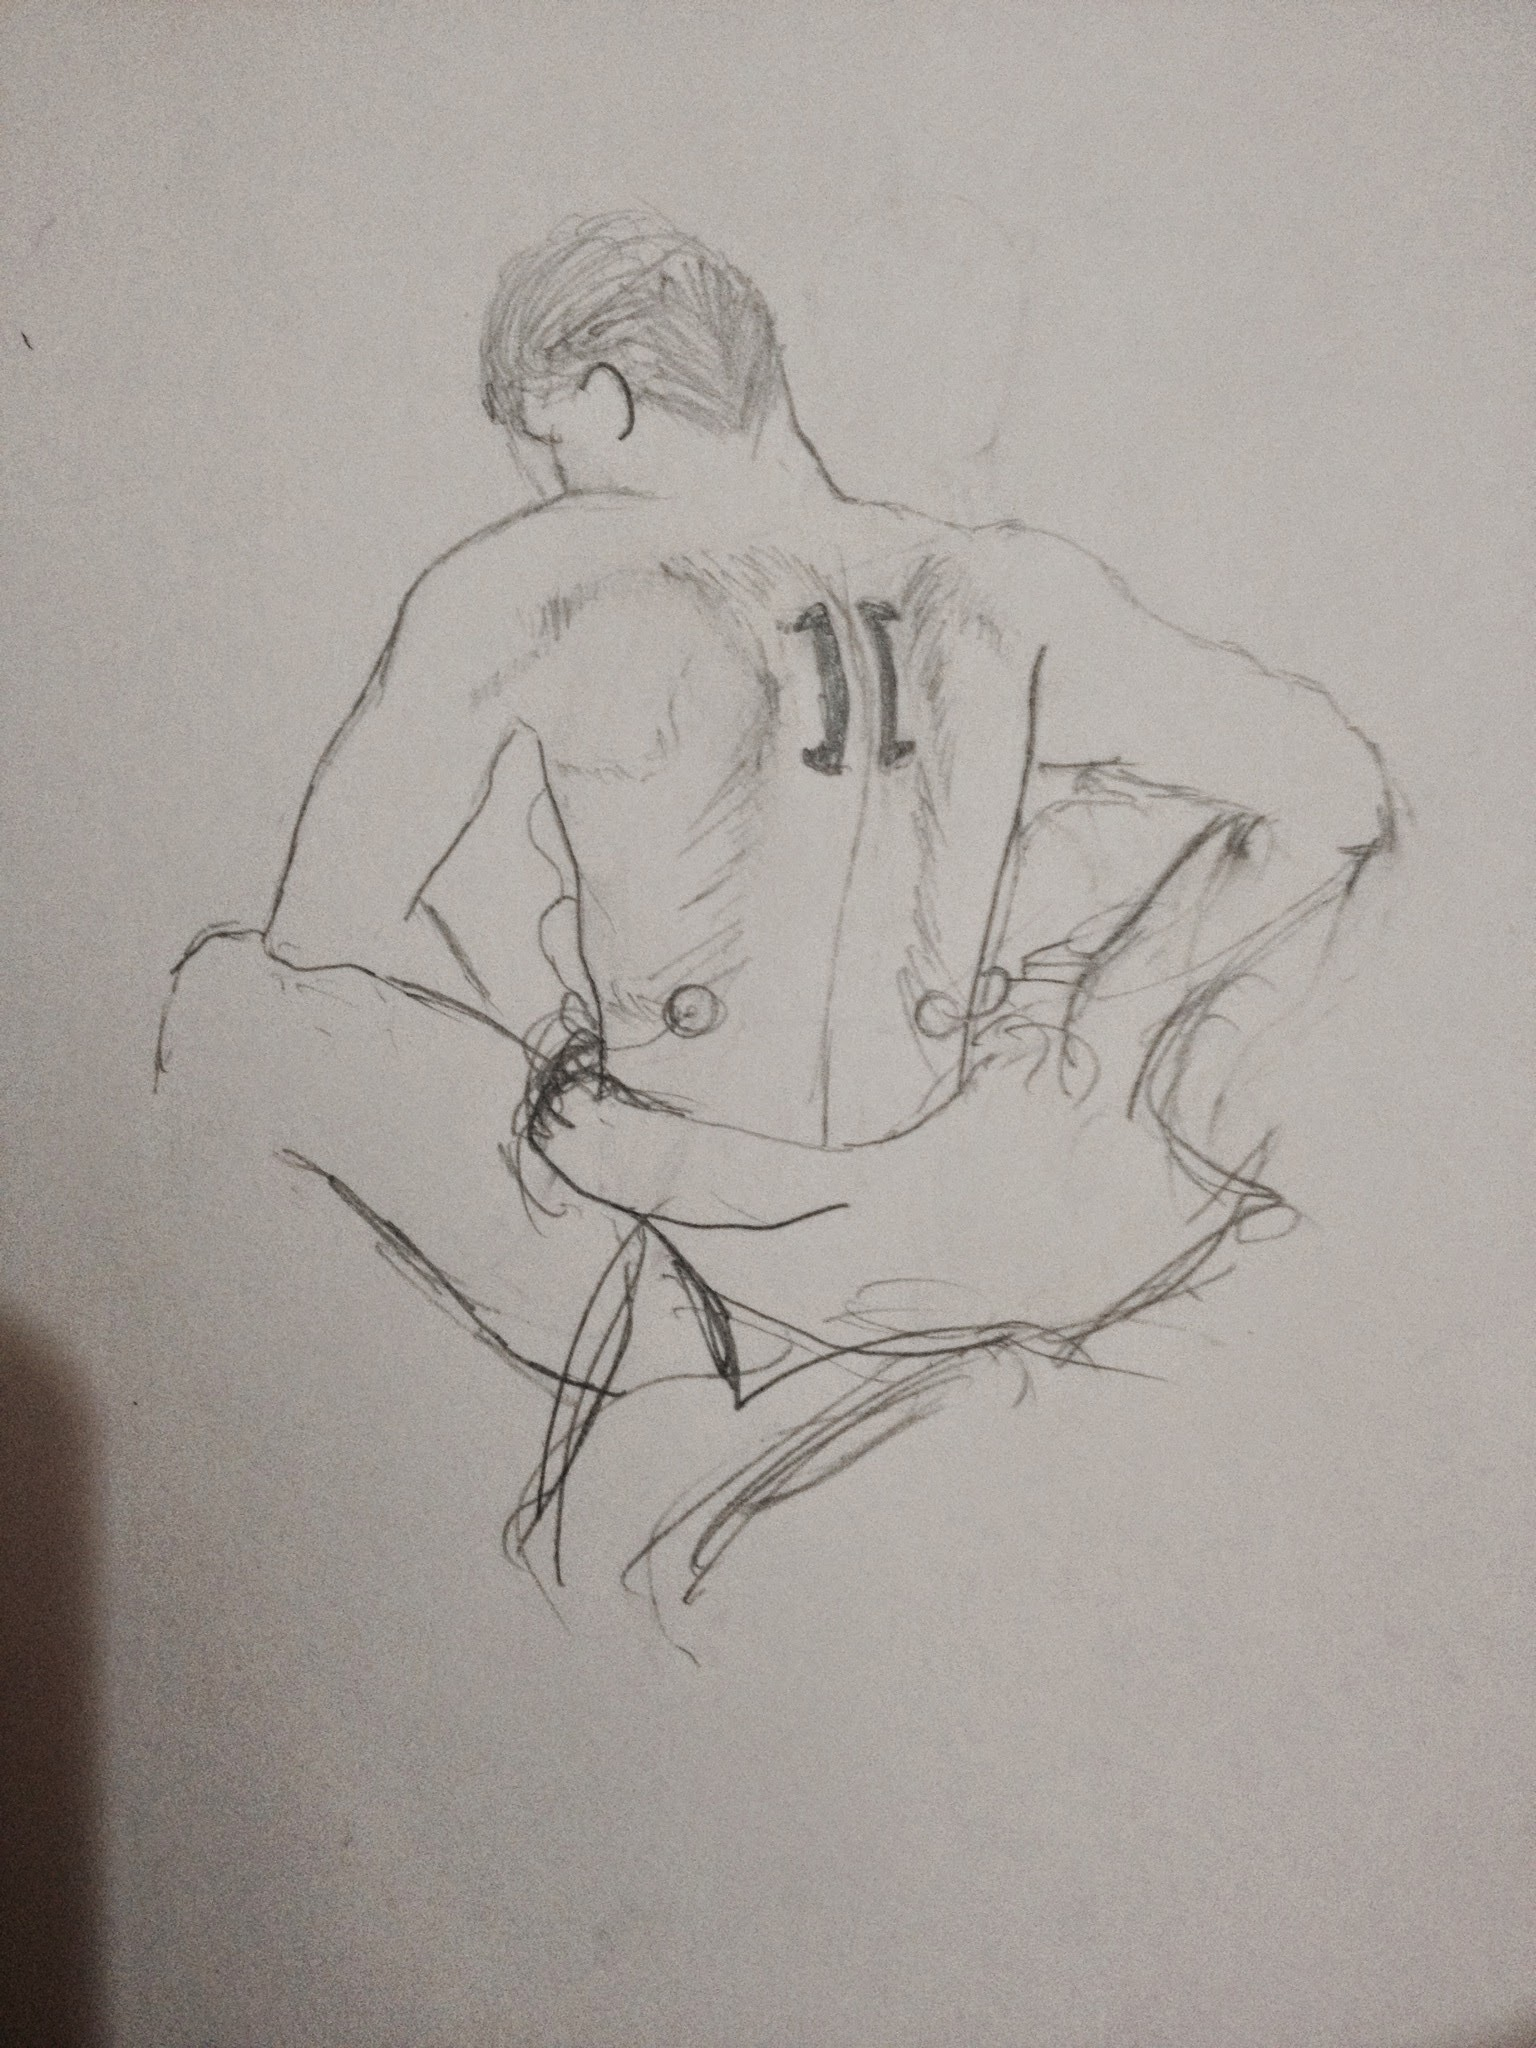
\includegraphics[width=12cm]{img/ch31_rook_ink.jpg}
\end{center}